\documentclass[11pt]{article}
\usepackage[a4paper, total={7in, 10in}]{geometry}
\usepackage{amsmath}
\usepackage{graphicx}
\usepackage{hyperref}
\graphicspath{ {./resources/} }
\usepackage[font=small,labelfont=bf]{caption} % Required for specifying captions to tables and figures
\usepackage[T1]{fontenc}
\usepackage[utf8]{inputenc}


\title{Scientific Computing - Condition and Stability}
\author{Mateusz Pełechaty}
\date{23 October 2022}%
\begin{document}
\maketitle


\section{Exercise 1}
Repeat exercise 5 from previous assignment list, but delete last $9$ in $x_4$ and last $7$ in $x_5$. What influence does it have on the results?
\subsection{Solution and results}
Previously 
\begin{align*}
x &= [2.718281828, -3.141592654, 1.414213562, 0.5772156649, 0.3010299957]\\
y &= [1486.2497, 878366.9879, -22.37492, 4773714.647, 0.000185049]
\end{align*}
As stated in assignment, we will use 
\begin{align*}
x' = [2.718281828, -3.141592654, 1.414213562, 0.577215664, 0.301029995]
\end{align*}

\begin{table}[!ht]
    \centering
    \caption{Scalar product $x\cdot y$ with different $x$ and precision}
    \begin{tabular}{|l|l|l|l|l|}
    \hline
        ~ & Float32 $x$ & Float32 $x'$ & Float64 $x$ & Float64 $x'$ \\ \hline
        Front & -0.4999443 & -0.4999443 & 1.0251881368296672e-10 & -0.004296342739891585 \\ \hline
        Back & -0.4543457 & -0.4543457 & -1.5643308870494366e-10 & -0.004296342998713953 \\ \hline
        Big To Small & -0.5 & -0.5 & 0.0 & -0.004296342842280865 \\ \hline
        Small to Big & -0.5 & -0.5 & 0.0 & -0.004296342842280865 \\ \hline
    \end{tabular}
\end{table}
\subsection{Conclusions}
As we can see small changes in data completely changes solution. Thus we can observe that calculating scalar product is ill-conditioned problem.

\section{Exercise 2}
\subsection{Draw graph of $f(x) = e^x ln(1+e^{-x})$ in any two graphing tools. }

\begin{minipage}{0.49\linewidth}
    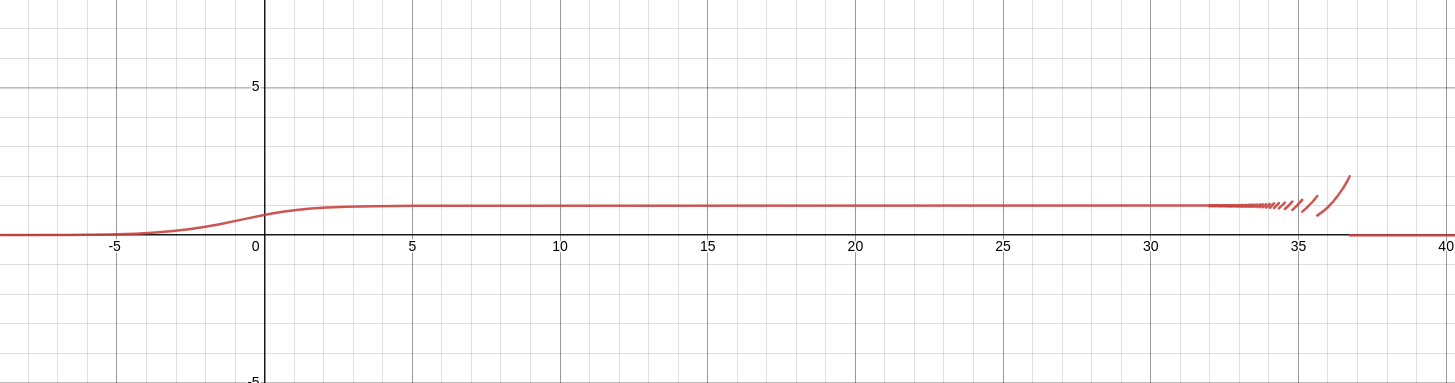
\includegraphics[scale=0.25]{ex2/desmos}
    \captionof{figure}{Desmos}
\end{minipage}\\
\hfill
\begin{minipage}{0.49\linewidth}
    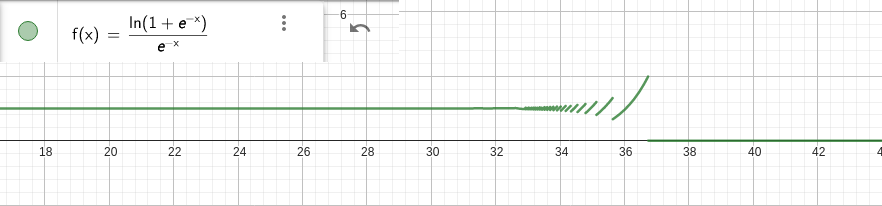
\includegraphics[scale=0.5]{ex2/geogebra}
    \captionof{figure}{Geogebra}
\end{minipage}

As we can see, for $30 < x < 37$, graph go wild and for $x\geq 37: f(x) = 0$
\subsection{Calculate $\lim_{x->\infty} f(x)$}
$$lim_{x->\infty}f(x) = lim_{x->\infty} e^xln(1+e^{-x}) = lim_{x->\infty} \frac{ln(1+e^{-x})}{e^{-x}} = (\star)$$
Note that $$lim_{x->\infty} ln(1+e^{-x}) = lim_{x->\infty} e^{-x} = 0$$
Because of it we can use L'Hôpital's rule.  
Let's calculate derivatives.
\begin{align*} 
\frac{d}{dx}ln(1+e^{-x}) &= \frac{-e^{-x}}{1+e^{-x}} = \frac{-1}{e^x + 1} \\
\frac{d}{dx}e^{-x} &= -e^{-x}
\end{align*} 
With this we can continue
$$(\star) = lim_{x->\infty} \frac{-1}{e^x + 1} \cdot \frac{-1}{e^{-x}} = lim_{x->\infty} \frac{1}{1 + e^{-x}} = \frac{1}{1+0} = 1$$  
So $\lim_{x->\infty} f(x) = 1$
\subsection{Conclusions}
Problem is ill-conditioned, because on the graphs small rounding errors change results of graph when $30< x < 37$. 
After it f(x) = 0, because $1+e^{-x} \approx 1$ when $x$ is big. Then $ln(1+e^{-x}) \approx ln(1) = 0$. \\ 
\textbf{Geogebra} and \textbf{Desmos} results doesn't match limit calculated by me.
\section{Exercise 3}
Consider task of solving system of linear equations
\begin{equation*}
    Ax = b
\end{equation*}
$A \in R^{N \times N}$ - Matrix of coefficients\\
$b$ - vector of right sides\\
Consider two methods of generating $A$\\
\textbf{a.} 
$A = H_n, n \in \{1,2,3,\hdots,20\}$, where $H_n$ is Hilbert's of $n$ degree generated by $A$=hilb(n)\\
\textbf{b.} 
$A = R_n, n \in \{5,10,20\}$, where $R_n$ is random matrix of $n$ degree generated 
with given condition $c \in \{1, 10, 10^3, 10^7, 10^{12}, 10^{16}\}$ generated by function $A$=matcond($n$, $c$)\\
Vector $b$ is given as $b = Ax$, where $x = (1,\dots,1)^T$
\subsection{Solve $Ax = b$ with $x = \frac{b}{A}$}
Results can be found in \textbf{Table 2} 
\begin{table}[!ht]
    \centering
    \caption{Hilbert's Matrix}
    \begin{tabular}{|l|l|l|l|l|}
    \hline
        n & cond(A) & rank(A) & A$\backslash$b error & inv(A)*b error \\ \hline
        1 & 1.0 & 1 & 0.0 & 0.0 \\ \hline
        2 & 19.28147006790397 & 2 & 5.661048867003676e-16 & 1.4043333874306803e-15 \\ \hline
        3 & 524.0567775860644 & 3 & 8.022593772267726e-15 & 0.0 \\ \hline
        4 & 15513.73873892924 & 4 & 4.137409622430382e-14 & 0.0 \\ \hline
        5 & 476607.2502425855 & 5 & 1.6828426299227195e-12 & 3.3544360584359632e-12 \\ \hline
        6 & 1.4951058642254734e7 & 6 & 2.618913302311624e-10 & 2.0163759404347654e-10 \\ \hline
        7 & 4.753673567446793e8 & 7 & 1.2606867224171548e-8 & 4.713280397232037e-9 \\ \hline
        8 & 1.5257575538060041e10 & 8 & 6.124089555723088e-8 & 3.07748390309622e-7 \\ \hline
        9 & 4.9315375594102344e11 & 9 & 3.8751634185032475e-6 & 4.541268303176643e-6 \\ \hline
        10 & 1.602441698742836e13 & 10 & 8.67039023709691e-5 & 0.0002501493411824886 \\ \hline
        11 & 5.222701316549833e14 & 10 & 0.00015827808158590435 & 0.007618304284315809 \\ \hline
        12 & 1.7515952300879806e16 & 11 & 0.13396208372085344 & 0.258994120804705 \\ \hline
        13 & 3.1883950689209334e18 & 11 & 0.11039701117868264 & 5.331275639426837 \\ \hline
        14 & 6.200786281355982e17 & 11 & 1.4554087127659643 & 8.71499275104814 \\ \hline
        15 & 3.67568286586649e17 & 12 & 4.696668350857427 & 7.344641453111494 \\ \hline
        16 & 7.046389953630175e17 & 12 & 54.15518954564602 & 29.84884207073541 \\ \hline
        17 & 1.249010044779401e18 & 12 & 13.707236683836307 & 10.516942378369349 \\ \hline
        18 & 2.2477642911280653e18 & 12 & 10.257619124632317 & 24.762070989128866 \\ \hline
        19 & 6.472700911391398e18 & 13 & 102.15983486270827 & 109.94550732878284 \\ \hline
        20 & 1.1484020388436145e18 & 13 & 108.31777346206205 & 114.34403152557572 \\ \hline
    \end{tabular}
\end{table}
\subsubsection{Conclusions}
We can see that in Hilbert's Matrix, $cond(A) = \theta(2^n)$ and because of it, both methods of generating solution has got huge rounding errors. 
We can guess that solving system of equations is ill-conditioned problem
\subsection{Solve $Ax = b$ with $x = A^{-1} \cdot b$}
\subsubsection{Results}
Results can be found in \textbf{Table 3} 
\begin{table}[!ht]
    \centering
    \caption{Random Matrix}
    \begin{tabular}{|l|l|l|l|l|l|}
    \hline
        n & c & cond(A) & rank(A) & A$\backslash$b error & inv(A)*b error \\ \hline
        5 & 1.0 & 1.0000000000000007 & 5 & 2.3288234633381846e-16 & 1.9860273225978183e-16 \\ \hline
        5 & 10.0 & 10.000000000000005 & 5 & 3.1401849173675503e-16 & 9.930136612989092e-17 \\ \hline
        5 & 1000.0 & 999.9999999998918 & 5 & 1.7587138213947747e-14 & 2.7747580858440746e-14 \\ \hline
        5 & 1.0e7 & 1.0000000002864836e7 & 5 & 1.1200819603238923e-10 & 7.917097832969997e-11 \\ \hline
        5 & 1.0e12 & 9.999750894774873e11 & 5 & 9.330538290671272e-6 & 8.986830894004628e-6 \\ \hline
        5 & 1.0e16 & 1.873964439700235e16 & 4 & 0.2958796386644769 & 0.2942316529964103 \\ \hline
        10 & 1.0 & 1.0000000000000013 & 10 & 2.4575834280036907e-16 & 1.4043333874306804e-16 \\ \hline
        10 & 10.0 & 10.000000000000002 & 10 & 3.274687455368547e-16 & 3.3857251850959236e-16 \\ \hline
        10 & 1000.0 & 999.9999999999555 & 10 & 4.6641419326660214e-14 & 4.9392224007846006e-14 \\ \hline
        10 & 1.0e7 & 1.000000000641046e7 & 10 & 1.9222994028809006e-10 & 1.7540944047859128e-10 \\ \hline
        10 & 1.0e12 & 9.999829164270026e11 & 10 & 1.1469317000942926e-5 & 9.060690243558819e-6 \\ \hline
        10 & 1.0e16 & 6.36137650086178e15 & 9 & 0.3067271248359218 & 0.28474392278413946 \\ \hline
        20 & 1.0 & 1.0000000000000018 & 20 & 4.852068387831067e-16 & 5.01447318807467e-16 \\ \hline
        20 & 10.0 & 9.999999999999991 & 20 & 5.4672143489065705e-16 & 4.902612130890297e-16 \\ \hline
        20 & 1000.0 & 1000.0000000000065 & 20 & 1.1644117316690922e-15 & 2.6700806038273252e-15 \\ \hline
        20 & 1.0e7 & 1.000000000092331e7 & 20 & 1.3006518187937346e-10 & 1.4732691292968656e-10 \\ \hline
        20 & 1.0e12 & 9.999657722483511e11 & 20 & 6.126439881933294e-6 & 9.331277994518528e-6 \\ \hline
        20 & 1.0e16 & 1.346974920376682e16 & 19 & 0.2891037414898818 & 0.31773928298705056 \\ \hline
    \end{tabular}
\end{table}
\subsubsection{Conclusions}
For $c=k,  k \in \{1, 10, 10^3, 10^7, 10^{12}, 10^{16}\}$ we get very similar results no matter what $n$ it is.
It shows that what is important is condition indicator.
\section{Exercise 4}
In this exercise we will refer to\\ 
$P(x)$ as to Wilkinson's polynomial in it's general form.\\
$p(x)$ as to Wilkinson's polynomial in factorial form
\subsection{Use roots function from Polynomials to compute roots of $P(x)$\\
Compare results with real roots by computing $|P(z_k)|$, $|p(z_k)|$, $|z_k - k|$ and explain discrepancies.}
\subsubsection{Results}
Results can be found in \textbf{Table 4}
\begin{table}[!ht]
    \centering
    \caption{Results of 4.1}
    \begin{tabular}{|l|l|l|l|l|}
    \hline
        $k$ & $z_k$ & $|P(z_k)|$ & $|p(z_k)|$ & $|z_k-k|$ \\ \hline
        1 & 0.9999999999996989 & 35696.50964788257 & 5.518479490350445e6 & 3.0109248427834245e-13 \\ \hline
        2 & 2.0000000000283182 & 176252.60026668405 & 7.37869762990174e19 & 2.8318236644508943e-11 \\ \hline
        3 & 2.9999999995920965 & 279157.6968824087 & 3.3204139316875795e20 & 4.0790348876384996e-10 \\ \hline
        4 & 3.9999999837375317 & 3.0271092988991085e6 & 8.854437035384718e20 & 1.626246826091915e-8 \\ \hline
        5 & 5.000000665769791 & 2.2917473756567076e7 & 1.8446752056545688e21 & 6.657697912970661e-7 \\ \hline
        6 & 5.999989245824773 & 1.2902417284205095e8 & 3.320394888870117e21 & 1.0754175226779239e-5 \\ \hline
        7 & 7.000102002793008 & 4.805112754602064e8 & 5.423593016891273e21 & 0.00010200279300764947 \\ \hline
        8 & 7.999355829607762 & 1.6379520218961136e9 & 8.262050140110275e21 & 0.0006441703922384079 \\ \hline
        9 & 9.002915294362053 & 4.877071372550003e9 & 1.196559421646277e22 & 0.002915294362052734 \\ \hline
        10 & 9.990413042481725 & 1.3638638195458128e10 & 1.655260133520688e22 & 0.009586957518274986 \\ \hline
        11 & 11.025022932909318 & 3.585631295130865e10 & 2.24783329792479e22 & 0.025022932909317674 \\ \hline
        12 & 11.953283253846857 & 7.533332360358197e10 & 2.886944688412679e22 & 0.04671674615314281 \\ \hline
        13 & 13.07431403244734 & 1.9605988124330817e11 & 3.807325552826988e22 & 0.07431403244734014 \\ \hline
        14 & 13.914755591802127 & 3.5751347823104315e11 & 4.612719853150334e22 & 0.08524440819787316 \\ \hline
        15 & 15.075493799699476 & 8.21627123645597e11 & 5.901011420218566e22 & 0.07549379969947623 \\ \hline
        16 & 15.946286716607972 & 1.5514978880494067e12 & 7.010874106897764e22 & 0.05371328339202819 \\ \hline
        17 & 17.025427146237412 & 3.694735918486229e12 & 8.568905825736165e22 & 0.025427146237412046 \\ \hline
        18 & 17.99092135271648 & 7.650109016515867e12 & 1.0144799361044434e23 & 0.009078647283519814 \\ \hline
        19 & 19.00190981829944 & 1.1435273749721195e13 & 1.1990376202371257e23 & 0.0019098182994383706 \\ \hline
        20 & 19.999809291236637 & 2.7924106393680727e13 & 1.4019117414318134e23 & 0.00019070876336257925 \\ \hline
    \end{tabular}
\end{table}
\subsubsection{Conclusions}
\textit{roots} function didn't compute roots numbered from 1 to 20. This is because coefficients of Wilkinson's Polynomial at lower exponents are 18 digits long and Float64 precision is $\approx 16$ digits.
Because of it Polynomial's coefficients are saved with rounding error. By looking at the table we can also guess that problem of computing roots is ill-conditioned. Small changes made by rounding error, make that $|p(z_k)|$ is nowhere near 0
\subsection{Swap coeffincients from $-210$ to $-210-2^{-23}$. Explain results}
\subsubsection{Results can be found in \textbf{Table 5}}
\begin{table}[!ht]
    \centering
    \caption{Coefficients after swapping}
    \begin{tabular}{|l|l|}
    \hline
        k & z'\_k \\ \hline
        1 & 0.9999999999998357 + 0.0im \\ \hline
        2 & 2.0000000000550373 + 0.0im \\ \hline
        3 & 2.99999999660342 + 0.0im \\ \hline
        4 & 4.000000089724362 + 0.0im \\ \hline
        5 & 4.99999857388791 + 0.0im \\ \hline
        6 & 6.000020476673031 + 0.0im \\ \hline
        7 & 6.99960207042242 + 0.0im \\ \hline
        8 & 8.007772029099446 + 0.0im \\ \hline
        9 & 8.915816367932559 + 0.0im \\ \hline
        10 & 10.095455630535774 - 0.6449328236240688im \\ \hline
        11 & 10.095455630535774 + 0.6449328236240688im \\ \hline
        12 & 11.793890586174369 - 1.6524771364075785im \\ \hline
        13 & 11.793890586174369 + 1.6524771364075785im \\ \hline
        14 & 13.992406684487216 - 2.5188244257108443im \\ \hline
        15 & 13.992406684487216 + 2.5188244257108443im \\ \hline
        16 & 16.73074487979267 - 2.812624896721978im \\ \hline
        17 & 16.73074487979267 + 2.812624896721978im \\ \hline
        18 & 19.5024423688181 - 1.940331978642903im \\ \hline
        19 & 19.5024423688181 + 1.940331978642903im \\ \hline
        20 & 20.84691021519479 + 0.0im \\ \hline
    \end{tabular}
\end{table}
\subsubsection{Conclusions}
If the coefficient of $x^{19}$ is decreased by $2^{-23}$ then some roots collided to double root. Leading to complex number and it's conjugated version.
This further proves that Wilkinson's polynomial is very ill-conditioned.  
\section{Exercise 5}
Consider following reccurence equation that represents population growth
\begin{equation}
    p_{n+1} := p_n + rp_n(1-p_n), n \in \{0, 1, 2, \dots\}
\end{equation}
    $r$ - constant\\
    $r(1-p_n)$ - coefficient of population growth\\
    $p_0$ - starting size of population as a percent of maximum population size
\subsection{Calculate $p_{40}$ for $p_0=0.01$ and $r=3$. 
Then calculate $p_{10}$. Then let $p'_{10} := trunc(p_{10}, 3)$ and compute $p'_{40}$.
Compare $p_{40}$ and $p'_{40}$}
\subsubsection{Results}
Results can be found on \textbf{Table 6}
\begin{table}[h]
    \centering
    \caption{5.1 Difference between normal and interrupted iteration of $p$}
    \begin{tabular}{|l|l|l|l|}
    \hline
        i & $p_i$ & $p'_i$ & $|p_i - p'_i|$ \\ \hline
        9 & 0.21559286 & 0.21559286 & 0.0 \\ \hline
        10 & 0.7229306 & 0.722 & 0.0009306073 \\ \hline
        11 & 1.3238364 & 1.3241479 & 0.00031149387 \\ \hline
        12 & 0.037716985 & 0.036488414 & 0.0012285709 \\ \hline
        13 & 0.14660022 & 0.14195944 & 0.004640773 \\ \hline
        14 & 0.521926 & 0.50738037 & 0.0145456195 \\ \hline
        15 & 1.2704837 & 1.2572169 & 0.013266802 \\ \hline
        16 & 0.2395482 & 0.28708452 & 0.047536314 \\ \hline
        17 & 0.7860428 & 0.9010855 & 0.11504269 \\ \hline
        18 & 1.2905813 & 1.1684768 & 0.122104526 \\ \hline
        19 & 0.16552472 & 0.577893 & 0.4123683 \\ \hline
        \vdots & \vdots & \vdots & \vdots \\ \hline
        39 & 1.2652004 & 0.3839622 & 0.88123816 \\ \hline
        40 & 0.25860548 & 1.093568 & 0.8349625 \\ \hline
    \end{tabular}
\end{table}

\subsection{Calculate $p_{40}$ for $p_0=0.01$ and $r=3$ in Float32 and Float64. Compare the results}
\subsubsection{Results}
Results can be found on \textbf{Table 7}
\begin{table}[h]
    \centering
    \caption{5.2 Difference between calculating $pi$ with different precisions $p$}
    \begin{tabular}{|l|l|l|l|}
    \hline
        i & Float32 & Float64 & |Float32 - Float64| \\ \hline
        0 & 0.01 & 0.01 & 2.2351741811588166e-10 \\ \hline
        1 & 0.0397 & 0.0397 & 1.4781951912512525e-9 \\ \hline
        2 & 0.15407173 & 0.15407173000000002 & 3.3555221379266698e-9 \\ \hline
        3 & 0.5450726 & 0.5450726260444213 & 1.089778434160138e-8 \\ \hline
        4 & 1.2889781 & 1.2889780011888006 & 9.863419747624391e-8 \\ \hline
        5 & 0.1715188 & 0.17151914210917552 & 3.3946635324966223e-7 \\ \hline
        \vdots & \vdots & \vdots & \vdots \\ \hline
        37 & 1.0813814 & 0.6822410727153098 & 0.39914036744734893 \\ \hline
        38 & 0.81736827 & 1.3326056469620293 & 0.5152373779953545 \\ \hline
        39 & 1.2652004 & 0.0029091569028512065 & 1.262291219607769 \\ \hline
        40 & 0.25860548 & 0.011611238029748606 & 0.24699424216434318 \\ \hline
    \end{tabular}
\end{table}
\subsection{Conclusions}
In 5.1, at the beginning small discrepancy was made and that completely changed results for $p_40$.\\
In 5.2, discrepancies were made by rounding errors all the time. It also completely changed the sequences for $p_40$\\
Overall by looking at these examples we can say that sequence $p_n$ is unstable.
\section*{Exercise 6}
Consider reccurence equation
\begin{equation*}
    x_{n+1} := x_n^2 + c, n \in \{0, 1, 2, \dots\}
\end{equation*} 
where $c$ - constant\\
For the following data, compute $x_{40}$ and observe behaviour of generated sequences
\begin{table}[!ht]
    \centering
    \begin{tabular}{ccc}
    \hline
        ID & $c$ & $x_0$ \\ \hline
        1 & -2 & 1 \\ 
        2 & -2 & 2 \\ 
        3 & -2 & 1.99999999999999 \\ 
        4 & -1 & 1 \\ 
        5 & -1 & -1 \\ 
        6 & -1 & 0.75 \\ 
        7 & -1 & 0.25 \\ \hline
    \end{tabular}
    \caption{Data to conduct experiment}
\end{table}
\subsection{Drawings}
We can look at graphic iterations of these sequences\\
\begin{minipage}{0.49\linewidth}
    \includegraphics[scale=0.7]{"ex6/c=-1.0_x0=-1.0"} 
    \captionof{figure}{$c=-1.0$, $x_0=-1.0$, 
    we can see that value didn't stabilise and flips between -1 and 0} 
\end{minipage}\\
\begin{minipage}{0.49\linewidth}
    \includegraphics[scale=0.7]{"ex6/c=-1.0_x0=0.25"} 
    \captionof{figure}{$c=-1.0$, $x_0=0.25$, 
    we can see that after some time $x_n$ started flipping between -1 and 0} 
\end{minipage}\\
\begin{minipage}{0.49\linewidth}
    \includegraphics[scale=0.7]{"ex6/c=-1.0_x0=0.75"} 
    \captionof{figure}{$c=-1.0$, $x_0=0.75$, 
    we can see that after some time $x_n$ started flipping between -1 and 0} 
\end{minipage}\\
\begin{minipage}{0.49\linewidth}
    \includegraphics[scale=0.7]{"ex6/c=-1.0_x0=1.0"} 
    \captionof{figure}{$c=-1.0$, $x_0=1.0$, 
    we can see that value didn't stabilise and flips between -1 and 0} 
\end{minipage}\\
\begin{minipage}{0.49\linewidth}
    \includegraphics[scale=0.7]{"ex6/c=-2.0_x0=1.0"} 
    \captionof{figure}{$c=-2.0$, $x_0=1.0$, 
    we can see that value doesn't stabilise and flips between -1 and 0} 
\end{minipage}\\
\begin{minipage}{0.49\linewidth}
    \includegraphics[scale=0.7]{"ex6/c=-2.0_x0=1.99999999999999"} 
    \captionof{figure}{$c=-2.0$, $x_0=1.99999999999999$, 
    $x_n$ will never stabilise, because for $x_n$ to become $-1$ or $2$, it first needs to be $-1$ or $2$ respectively.} 
\end{minipage}\\
\begin{minipage}{0.49\linewidth}
    \includegraphics[scale=0.7]{"ex6/c=-2.0_x0=2.0"} 
    \captionof{figure}{We can see that $x_n$ stabilised} 
\end{minipage}\\
\subsection{Conclusions}
For sequence to stabilise it needs to start in one of the fixed points. Fixed points $x$ are the ones that meet equation
$$x = x^2 + c$$
Otherwise it will never reach it.
We can even see on \textbf{Figure 8} that even small discrepancy in input data can make huge discrepancies later on.
Thus this problem is ill-conditioned.
\end{document}